\documentclass{beamer}
\mode<presentation>
{
  \usetheme{default}      % or try Darmstadt, Madrid, Warsaw, ...
  \usecolortheme{beaver} % or try albatross, beaver, crane, ...
  \usefonttheme{serif}  % or try serif, structurebold, ...
  \setbeamertemplate{navigation symbols}{}
  \setbeamertemplate{caption}[numbered]
} 
\usepackage{tabularx}
\usepackage{graphicx} 
\newcommand\T{\rule{0pt}{2.6ex}}       % Top strut 
\newcommand\B{\rule[-1.2ex]{0pt}{0pt}} % Bottom strut 
\usepackage[utf8]{inputenc}
\usepackage[]{algorithm2e}

%Information to be included in the title page:
\title{Learning Low-Dimensional Representations
of Medical Concepts \\
}
\author{YD Choi, Yi-I Chiu, David Sontag }
\institute{Courant Institute of Mathematical 
Sciences, New York University}
 
\begin{document}
 
\frame{\titlepage} 

\begin{frame}
\frametitle{Disclosure}
\begin{center}
The authors have no relationships 
with commercial interests.
\end{center}
\end{frame}

\begin{frame}
\frametitle{Low-Dimensional Representations of 
Medical Concepts}
\begin{center}
\begin{itemize}
\item The central objects of study are
low dimensional representations of medical 
concepts, also referred to as medical concept
embeddings.
\end{itemize}
\bigskip

\begin{figure}[t]
    \centering 
    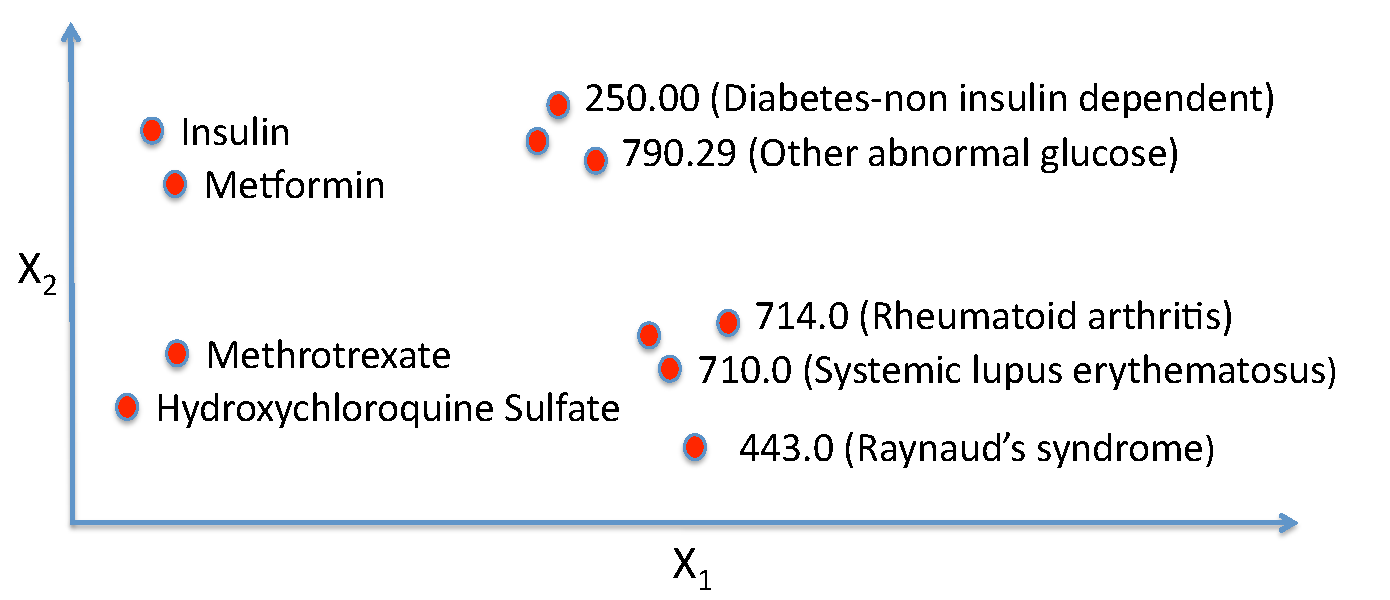
\includegraphics[width=.6\linewidth]{figs/illustration_of_embeddings.pdf}
    \caption{\centering 
\scriptsize Illustration a low-dimensional representation (in
      this case, 2 dimensions) of medical concepts. Similar concepts are close to each other in Euclidean space.
\label{fig:illustration_of_embeddings}}
\end{figure}
\end{center}
\end{frame}

\begin{frame}
\frametitle{Motivation: Why Medical Concept Embeddings?}
\begin{center}
\begin{itemize}
\item 
Learning distributed low-dimensional representations,
word embeddings, has proven particularly useful
in various language processing tasks, ranging from
simple language modeling to information extraction.

\bigskip

\item Many Deep Learning models in natural processing,
such as recurrent neural networks, 
rely on the concept of 
low dimensional representations.

\bigskip

\item The dimensionality of medical concepts, 
identified with standard medical ontologies are
roughly around $100,000$ (UMLS, ICD9, NDC, etc.),
which 
suffers from the same problem of curse of dimensionality. 

\end{itemize}
\end{center}
\end{frame}

\begin{frame}
\frametitle{Previous Work}
\begin{itemize}
\item Algorithmically, we leverage and modify 
the work of Mikolov et al., Word2Vec,
and Levy et al, SVD method with Shifted Positive
Pointwise Mutual Information.

\bigskip

\item There are previous works, specifically for
learning medical concept embeddings, using the
techniques above (DeVine et al., Minaro-Gimenez et al).
We will discuss them further in the
later section. 

\end{itemize}
\end{frame}

\begin{frame}
\frametitle{Outline}
\begin{center}
The talk will include two main parts:

\bigskip

\begin{itemize}
\item Description of the introduced embeddings: 
the distributions of interest 
and necessary algorithmic adjustments.

\bigskip

\item Quantitative analysis of the embeddings:
an identification of abstract properties
and their associated metrics.


\end{itemize}
\end{center}
\end{frame}

\begin{frame}
\frametitle{Three Types of Medical Concept Embeddings}
\begin{itemize}
\item Medical Concept Embeddings from Medical
Journals(Previous work; MCEMJ)

\bigskip

\item Medical Concept Embeddings from Medical Claims 
(New; MCEMC)

\bigskip

\item Medical Concept Embeddings from Clinical 
Narratives (New; MCECN)
\end{itemize}
\end{frame}

\begin{frame}
\frametitle{Background}
\begin{itemize}
\item In natural language processing, the key
information, that allows one to learn a sensible
set of embedding of words, is 
the distribution of nearby 
words, observed at the document level. 

\bigskip

\item With the distribution of nearby words, 
one can choose to train a neural network
that optimizes the prediction of nearby words,
or use techniques for 
producing low-dimensional factorization of matrices. 


\bigskip

\item Previous works of medical concept embeddings
naturally extend the idea by using the same idea,
but restricting the algorithm to medical texts
and only medically relevant terms. 

\end{itemize}
\end{frame}

\begin{frame}
\centering
We will instead focus on the distribution of 
temporally nearby medical concepts, within
available context of a given patient.

\end{frame}

\begin{frame}
\frametitle{Medical Concept Embeddings from
Medical \\ Claims (MCEMC)}
\begin{figure}[t]
    \centering 
    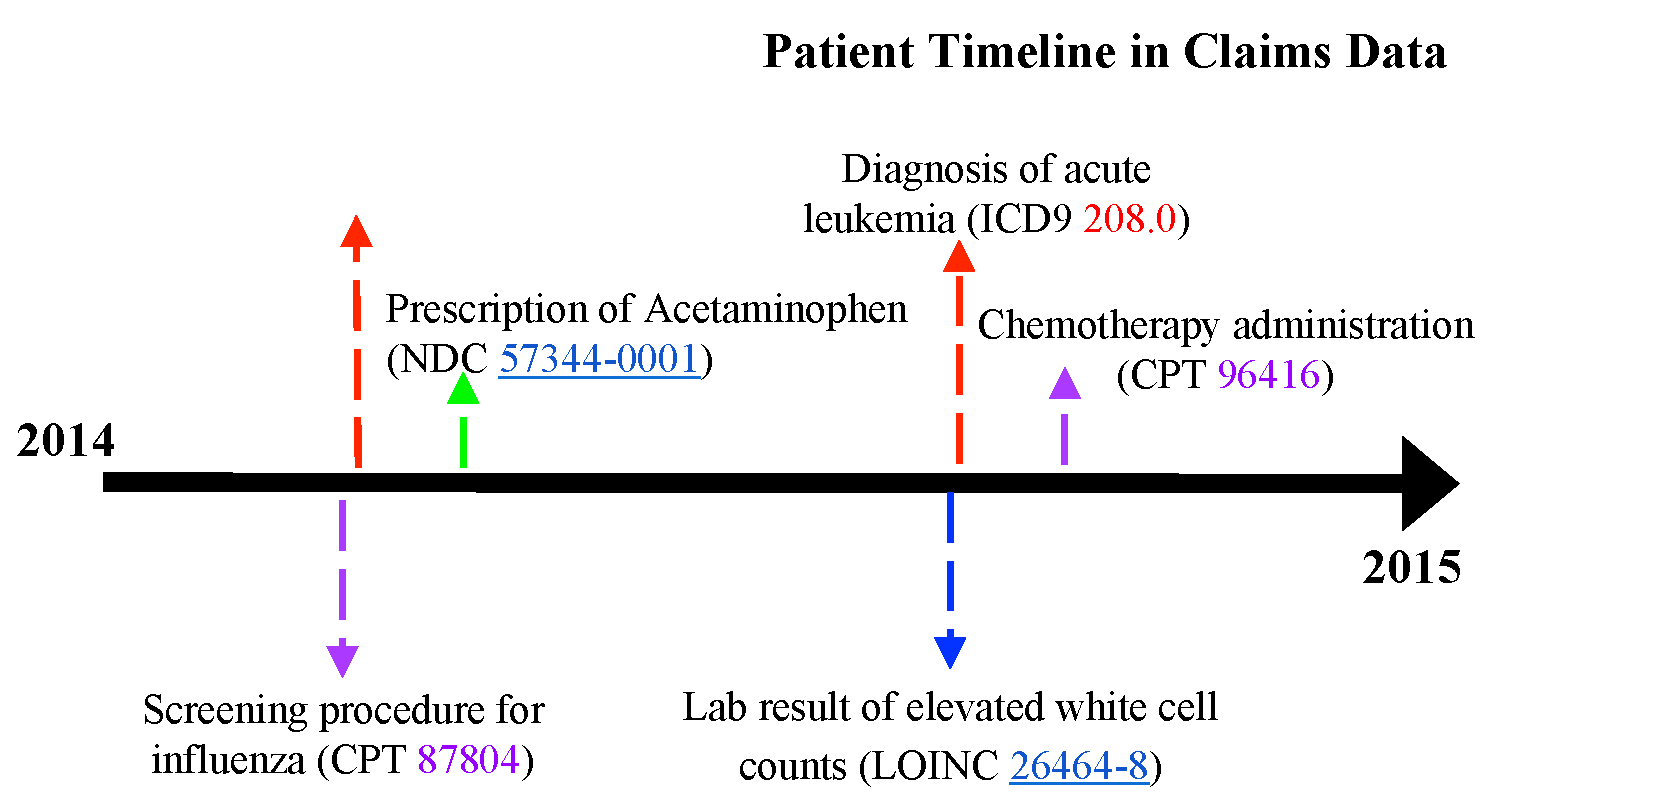
\includegraphics[width=0.8\linewidth]{figs/Figure1-claims-timeline.pdf}
    \caption{\scriptsize Illustration of the data used to learn
      embeddings of medical concepts, for a single patient.\label{fig:temporal}}
\end{figure}
\end{frame}

\begin{frame}
\frametitle{Medical Concept Embeddings from
Clinical \\ Narratives (MCECN)}
\begin{figure}[t]
    \centering 
    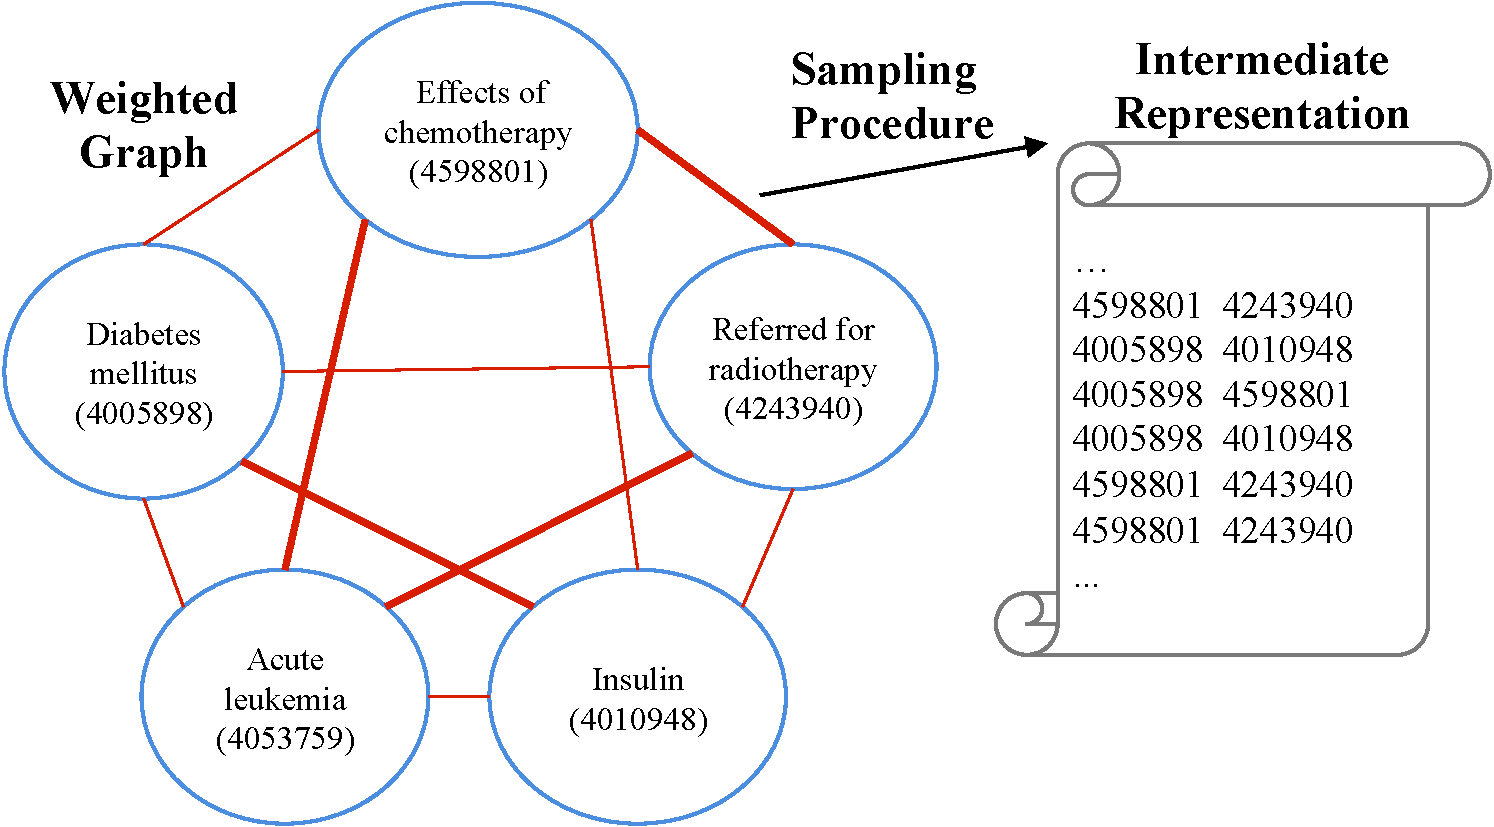
\includegraphics[width=0.8\linewidth]{figs/Figure1-transform.pdf}
    \caption{ \scriptsize
Shown on the left is the input, a weighted graph
of medical concept pairs with their
temporal frequencies from Shah et al.}  
\end{figure}
\end{frame}

\begin{frame}
\frametitle{Preliminary studies: the neighborhood
structures look different.}
\begin{itemize}
\item It is standard to look at the neighborhood
structures of word embeddings in natural language
processing community.

\bigskip

\item Even from our preliminary studies,
we qualitatively observed that there were significant differences in the respective neighborhood structures
among the embeddings.

\bigskip

\item For instance, in one set of embeddings, diagnosis
codes for various kinds of cancer formed a cluster, whereas in another set, a cluster
around lung cancer would include drugs and treatments related to lung cancer.

\end{itemize}
\end{frame}

\begin{frame}
\frametitle{Limitations of qualitative analysis}
\begin{itemize}
\item Although it is standard to do such analysis
by observing the selected subset of embeddings,
it is not entirely obvious, if the claim holds
true for the entire set of embeddings ($100,000$ 
medical concepts) 

\bigskip

\item What do we exactly mean by medically
related? 

\end{itemize}
\end{frame}

\begin{frame}
\begin{center}
Can we provide a concrete, quantitative methodology,
with which we could precisely characterize each set of embeddings?
\end{center}
\end{frame}

\begin{frame}
\frametitle{Call for Methodology: Two Abstract 
Properties}
\begin{center}
To address the issue, we introduce the notion of
two abstract properties to formalize the
intuition, that we gathered from the preliminary 
studies:

\bigskip

\begin{itemize}
\item The Conceptual Similarity Property

\bigskip

\item The Medical Relatedness Property
\end{itemize}
\end{center}
\end{frame}

\begin{frame}
\frametitle{dd}
\end{frame}

\begin{frame}
\frametitle{Definition of the 
Conceptual Similarity Property}

Concretely, we define the Medical Conceptual Similarity Measure (MCSM) 
of a set of concepts $V$
with respect to a conceptual type set $T$ induced by the UMLS (e.g.,
neoplastic process), parameterized by 
a size of the neighborhood $k$, as: %by $\text{MCSM}_{\text{UMLS}}(V,T,k)$, as
\begin{eqnarray*}
\text{MCSM}_{\text{UMLS}}(V,T,k) &=& \frac{1}{V(T)}\sum_{v \in V(T)} \sum_{i=1}^{k} \dfrac{ \mathtt{1}_{T}(v(i)) }{\log_2(i+1)},
\end{eqnarray*}
where $V(T)\subset V$ is the set of concepts of type $T$, $v(i)$ denotes the $i$th closest neighbor of the chosen medical concept $v$,
and $\mathtt{1}_{T}$ is an indicator function which is 1 if concept
$v(i)$ is of type $T$, and $0$ otherwise.
\end{frame}

\begin{frame}
\frametitle{Definition of 
the Medical Relatedness Property}
Concretely, for NDF-RT we define the Medical Relatedness Measure (MRM) of a set
of concepts $V$ 
with respect to a medical relation $R$, parameterized by
a size of the neighborhood $k$ and choice of a seed pair $s$, as: %denoted by $\text{MRM}_{\text{NDF-RT}}(V,R,k,s)$, as
\begin{eqnarray*}
\text{MRM}_{\text{NDF-RT}}(V,R,k,s) &=& \dfrac{1}{|V^*|}\sum_{v \in V^*} \mathtt{1}_{R}\Big(\bigcup_{i=1}^{k}(v-s)(i)\Big),
\end{eqnarray*}
where $V^*\subset V$ denotes the set of concepts for which NDF-RT
specifies at least one pharmacological substance with the given
relation, and $1_{R}$ is the indicator function which returns $1$ if
{\em any} of the medical concepts in the top-$k$ neighborhood of the
selected medical concept is an element with the given relation $R$, and  
$0$ otherwise. 
\end{frame}
\begin{frame}
\frametitle{Outline}
\end{frame}
\begin{frame}
\frametitle{The Article under Investigation}
\begin{table}[h!]
\begin{center}
\caption{\centering \scriptsize 
Medical conceptual similarity property comparison of MCEMJ and MCECN-SGD through  
$\text{MCSM}_{\text{UMLS}}$.} 
{
\tiny
\begin{tabular}{|c|c|c|}
    \hline      
                      & 
$\text{MCSM}_{\text{UMLS}}(\text{MCEMJ\cite{DeVine2014}},-,40)$ & 
$\text{MCSM}_{\text{UMLS}}(\text{MCECN-SGD},-,40)$\\ 
    \hline
    Pharmacologic Substance & {\bf 6.74 $\pm$ 3.21}  &  2.95 $\pm$ 2.15 \T \B  \\
    \hline
    Disease or Syndrome     & {\bf 5.41 $\pm$ 2.48}  &  4.28 $\pm$ 1.60 \T \B \\
    \hline
    Neoplastic Process      & {\bf 6.74 $\pm$ 3.47}  &  4.54 $\pm$ 0.11  \T \B \\
    \hline
    Clinical Drug           & {\bf 1.01 $\pm$ 0.12}  &  0.12 $\pm$ 0.18  \T \B \\
    \hline
    Finding                 & {\bf 2.85 $\pm$ 1.90}  &  2.15 $\pm$ 1.35  \T \B \\
    \hline
    Injury or Poisoning     & 2.67 $\pm$ 2.40  &  {\bf 2.92 $\pm$ 2.80}  \T \B \\
    \hline
\end{tabular}
}
%}
%\end{sc}
%\end{small}
\end{center}
\label{umls_dcg}
\end{table}

\end{frame}

\begin{frame}
\frametitle{The Article under Investigation}
\begin{table}[h!]
\caption{\centering
\scriptsize Display of a sub-computation for$\text{ MCSM}_{\text{UMLS}}(\text{MCECN},\text{Neoplastic Process}, 8)$.}
{
\tiny
\begin{center}
\begin{tabular}{|c|}
\hline
Neighbors of CUI 4003436 (Carcinoma, non-small-cell lung) [`Neoplastic Process'] 
\T \B \\ 
\hline
\textbf{4069419 (small cell carcinoma of lung, C0149925,  [`Neoplastic Process']) : 0.956} \T \B \\
\textbf{4394316 (carcinoma of lung, C0684249,  [`Neoplastic Process']) : 0.934} 
\T \B \\
\textbf{4125384 (malignant neoplasm of lung, C0242379,  [`Neoplastic Process']) : 0.929} \T \B \\
\textbf{4070138 (adenocarcinoma of lung (disorder), C0152013,  [`Neoplastic Process']) : 0.925} \T \B \\
4555365 (tarceva, C1135136,  [`Organic Chemical', `Pharmacologic Substance']) : 0.918 \T \B \\
4069342 (lung mass, C0149726,  [`Finding']) : 0.914 \T \B \\
4542086 (alimta, C1101816,  [`Organic Chemical', `Pharmacologic Substance']) : 0.903 \T \B \\
\textbf{4148168 (non-small cell lung cancer metastatic, C0278987,  [`Neoplastic Process']) : 0.900} \T \B \\
\hline
\end{tabular}
\end{center}
}
\end{table}
\end{frame}

\begin{frame}
\frametitle{the article under investigation}

\begin{table}[t]
\caption{\centering
\scriptsize Display of a sub-computation for $\text{MRM}_{\text{NDF-RT}}(\text{MCECN},\text{May-Treat},8,-)$. 
}{
\tiny
\begin{center}
\begin{tabular}{|c|} 
\hline
Neighbors of CUI 4003436 (Carcinoma, non-small-cell lung) [`Neoplastic Process'] 
\T \B \\ 
\hline
4069419 (small cell carcinoma of lung, C0149925,  [`Neoplastic Process']) : 0.956 \T \B \\
4394316 (carcinoma of lung, C0684249,  [`Neoplastic Process']) : 0.934 
\T \B \\
4125384 (malignant neoplasm of lung, C0242379,  [`Neoplastic Process']) : 0.929 \T \B \\
4070138 (adenocarcinoma of lung (disorder), C0152013,  [`Neoplastic Process']) : 0.925\T \B \\
\textbf{4555365 (tarceva, C1135136,  [`Organic Chemical', `Pharmacologic Substance']) : 0.918} \T \B \\
4069342 (lung mass, C0149726,  [`Finding']) : 0.914 \T \B \\
\textbf{4542086 (alimta, C1101816,  [`Organic Chemical', `Pharmacologic Substance']) : 0.903} \T \B \\
4148168 (non-small cell lung cancer metastatic, C0278987,  [`Neoplastic Process']) : 0.900 \T \B \\
\hline
\end{tabular}
\end{center}
}
\end{table}
\end{frame}

\begin{frame}
\frametitle{the article under investigation}
\begin{table}[t]
    \caption{\centering \scriptsize 
The Medical Relatedness Property comparison of various embeddings through $\text{MRM}_{\text{NDF-RT}}$.
    The results are of the form (neighbors/avg-seed/max-seed).\label{table:maytreat_mayprevent}}
{
\tiny
\begin{center}
    \begin{tabular}{|c|c|c|}
        \hline
                  & $\text{MRM}_{\text{NDF-RT}}(-,\text{May Treat},40)$  & $\text{MRM}_{\text{NDF-RT}}(-,\text{May Prevent},40)$\\
        \hline
        $\text{MCEMJ}_\text{r=5,d=200}$ \cite{DeVine2014} & 12.59\% / 31.56\% / 53.92\%   & 18.12\% / {\bf 35.20\%} / 55.88\% \T \\
        \hline
        $\text{MCEMC}_\text{month,ns20}$ & 10.93\% / 28.67\% / 57.01\%   & 5.88 \% / 29.45\% / {\bf 57.35\%} \T \\
        \hline
        $\text{MCEMC}_\text{month,hs}$ & 19.24\% / {\bf 37.68\% } / {\bf 60.57 \% }  & 8.82 \% / 30.20\% / {\bf 57.35\% }  \T \\
        \hline
        $\text{MCECN-SGD}_\text{1Bil,7d,ns20}$ & 36.81\% / 33.94\% / 57.48\%  & 27.94\% / 30.42\%  / 45.59\% \T \\
        \hline
        $\text{MCECN-SGD}_\text{10Bil,7d,ns20}$ & 38.72\% / 34.90\% / 57.95\%  & 32.95 \% / 31.99\% / 48.53\% \T \\
        \hline
        $\text{MCECN-SVD}_\text{7d,ns10}$ & {\bf 52.26\%} / 35.70 \% / 53.21\% & {\bf 39.71\%} / 32.32\% / 50.00\% \T \\
        \hline
    \end{tabular}
\end{center}
}
%    \end{sc}
%    \end{small}
%    \end{center}
\end{table}
\end{frame}

\begin{frame}
\frametitle{the article under investigation}
\begin{table}[h!]
    \caption{\centering \scriptsize The Medical Relatedness Property comparison of various embeddings through $\text{MRM}_{\text{CCS}}$.\label{table:disease_disease}}
    \begin{center}
\tiny
%    \begin{small}
%    \begin{sc}
{
    \begin{tabular}{|c|c|c|}
        \hline
                  & $\text{MRM}_{\text{CCS}}(-,\text{Fine-grained},40)$  & $\text{MRM}_{\text{CCS}}(-,\text{Coarse-grained},40)$ \\
        \hline
        $\text{MCEMJ}_\text{r=5,d=200}$ \cite{DeVine2014} & 0.2293   & 0.2490 \T \\
        \hline
        $\text{MCEMC}_\text{month,ns20}$ & 0.4127   & 0.4422 \T \\
        \hline
        $\text{MCEMC}_\text{month,hs}$ & {\bf 0.4536} & {\bf 0.4804 } \T \\
        \hline
        $\text{MCECN-SGD}_\text{1Bil,7d,ns20}$ & 0.2966 & 0.3319 \T \\
        \hline
        $\text{MCECN-SGD}_\text{10Bil,7d,ns20}$ & 0.3087 & 0.3420 \T \\
        \hline
        $\text{MCECN-SVD}_\text{7d,ns10}$ & 0.3461  & 0.3776 \T \\
        \hline
    \end{tabular}
}
%    \end{sc}
%    \end{small}
    \end{center}
\vspace{-1mm}
\end{table}
\end{frame}

\begin{frame}
\frametitle{the article under investigation}
\begin{table}[t]
\caption{\centering \scriptsize 
The neighborhood of the diagnosis code $710.0$ in the MCEMC. We display
the top $5$ neighbors for each type of code, filtering duplicates.\label{table:nn_diagnosis}}
\tiny
{
\begin{center}
\begin{tabular}{|c|c|}
\hline
& Nearest Neighbors of ICD9 710.0 (Systemic lupus erythematosus) in MCEMC \\
\hline
& {\bf Diagnoses (ICD9) } \T \\
\hline
1 & 695.4 (Lupus erythematosus) \T \\
2 & 710.9 (Unspecified diffuse connective tissue disease) \T \\
3 & 710.2 (Sicca syndrome) \T \\
4 & 795.79 (Other and unspecified nonspecific immunological findings) \T \\
5 & 443.0 (Raynaud's syndrome) \T \\
\hline
& {\bf Laboratory tests (LOINC) } \T \\
\hline
1 & 4498-2 (Complement C4 in Serum or Plasma) \T \\
2 & 4485-9 (Complement C3 in Serum or Plasma) \T \\
3 & 5130-0 (DNA Double Strand Ab) in Serum) \T \\
4 & 14030-1 (Smith Extractable Nuclear Ab+Ribonucleoprotein Extractable Nuclear Ab in Serum) \T \\
5 & 11090-8 (Smith Extractable Nuclear Ab in Serum) \T \\
\hline
& {\bf Drugs (NDC) } \T \\
\hline
1 & 00378037301 (Hydroxychloroquine Sulfate 200mg) \T \\
2 & 00024156210 (Plaquenil 200mg) \T \\
3 & 51927105700 (Fluocinolone Acetonide Miscell Powder) \T \\
4 & 00062331300 (All-flex Contraceptive Diaphragm Arcing Spring Ortho All-flex 80mm) \T \\
5 & 00054412925 (Cyclophosphamide 25mg) \T \\
\hline
\end{tabular}
\end{center}
}
\end{table}
\end{frame}

\begin{frame}
\frametitle{the article under investigation}
\begin{table}[t]
\caption{\centering \scriptsize
 A few neighborhood
  examples from MCECN illustrating genotypic-phenotypic relations.\label{table:genotype-examples}}
{ \tiny
\begin{center}
\begin{tabular}{|c|c|} 
\hline
 {\bf (cd52, C2733653)} &  {\bf (bcl1, C2599665)} \T \B \\ 
\hline
(cd52 protein, human, C0376272) &  (cyclins, C0079183) \T \\
(mycosis fungoides/sezary syndrome nos, C0862196) &   (proliferating cell nuclear antigen, C0072108) \T \\
(t-cell receptor, C0034790) &  (lymphoplasmacytic lymphoma, C2700641) \T \\
 (lymphoma, t-cell, cutaneous, C0079773) & (paired box 5 protein, C0167636) \T \\
 (pralatrexate, C1721300) &   (cyclin d1, C0174680) \T \\
\hline
{\bf (jak2 mutation, C2827348)} & {\bf (kras mutation, C2747837) }  \T \B \\
\hline
 (refractory anemia with ringed sideroblasts, C1264195) & (mesothelioma, C0025500) \T \\
(large platelets (finding), C1148412) &  (cdx2 protein, human, C1505661) \T \\
 (anagrelide, C0051809) &  (cdx2 antigen, C1829706) \T \\
 (hypercellular bone marrow, C1334068)  & (pleural mass, C1709576) \T \\
 (myeloid metaplasia, C0027013) & (braf protein, human, C1259929) \T \\
\hline
\end{tabular}
\end{center}
}
\end{table}
\end{frame}

\begin{frame}
\frametitle{the article under investigation}
\end{frame}

\begin{frame}
\frametitle{the article under investigation}
\end{frame}

\end{document}
